This chapter introduces the concepts necessary to understanding the subject of this thesis.
We aim to:
\begin{itemize}
    \item present the central pieces of an \emph{agent-based approach} in artificial intelligence: agent and environment;
    \item explain how we can reason about problems using this paradigm;
    \item introduce key concepts in the field of \emph{reinforcement learning (RL)};
    \item describe \emph{Q-learning} and how we can use neural networks to improve the classic algorithm;
    \item exemplify a successful application of this approach.
\end{itemize}

\section{Intelligent Agents} \label{agents-intro}
This section aims to provide a short introduction to the central pieces of an \emph{agent-based approach} in artificial intelligence: agent and environment.
Understanding how to formulate relevant problems in terms of agents learning from controlled environments is necessary to the core technique presented in this paper -- reinforcement learning (presented in \ref{reinforcement-learning}).

The concept of rational agent is central to the study of artificial intelligence. 
It is a natural evolution to the \textit{laws of thought} approach in AI (using a set of logical rules to derive new knowledge).

As pointed out in \cite{aima}, inference does not capture all of rationality.
As complex environments imply \textit{uncertain situations} (where there is no provably correct choice to make), a finite set of rules can prove inadequate.
The agent-based approach captures a more complete definition of rationality by shifting focus from making correct inferrences to producing \emph{efficient behaviour}.

\subsection{Agent Function and Agent Program}
According to \cite{aima}, an \textbf{agent} is simply something that percieves and acts in an environment.
An agent can be split into two major components, each fulfilling a fundamental function:
\emph{perceptors} (sensors) manage \emph{perception} and \emph{actuators} act upon the environment.
This is the simplest useful division. We present a more elaborate division later, in Section \ref{learning-agents}.

It is sometimes useful to reason about agents in a mathematical space.
For this, there exists the concept of \emph{agent function}.
An \textbf{agent function} maps what the agent percieves (every ``snapshot'' of perception, called a \emph{percept}) to an action.
Outside the world of very small, ideal examples, any agent function can be considered \emph{infinite}.
The implementation of an agent function is an \textbf{agent program}, which is what AI is actually concerned with building and perfecting.
This implementation is, of course, finite.

The term \emph{agent} \textbf{can} designate physical robots working in real-life environments.
However, in this paper we use the term \textit{agent} to refer exclusively to softbots (or software robots).
The problem that we solve can be entirely modeled in a virtual space.

\subsection{Task Environments}
Simply put, \textbf{task environments} are a way to express a problem to which an agent is the solution.
The design of the agent depends on the attributes of its environment.

In this paradigm, we can decompose a task into several subcomponents, often abbreviated \textbf{PEAS} \cite{aima}, comprising of:
\begin{enumerate}
    \item \textbf{performance measure}, a function which measures the performance of the agent;
    \item \textbf{environment}, the ``world'' the agents interacts with;
    \item \textbf{actuators}, the agent's means of action;
    \item \textbf{sensors}, the agent's means of perception;
\end{enumerate}

The \textbf{performance measure} has many possible representations, depending on the problem.
Its primary purpose is to measure how effective the behaviour of the agent is, with regard to the given goals.
In reinforcement learning, we measure this effectiveness using a \textbf{reward function}.
We will elaborate on this in our section on reinforcement learning (Section \ref{reinforcement-learning}).

\subsubsection{Environment Classification}

Modeling real-world use cases requires understanding the vast diversity of environments.
In the following paragraphs, we present some \textbf{classification criteria} for task environments that are also provided in \cite{aima}.

\textbf{Observability} can be \emph{full} or \emph{partial}.
In a fully observable environment, the agent has full information of all the relevant aspects of the world (for example, a chess-playing agent sees the entire chessboard).
The latter means the agent operates with restricted information.
Many real-world problems have partial observability due to sensor noise or memory/CPU constraints.

\textbf{Single- or multi-agent}.
Multi-agent environments are a tool for studying emergent behaviour, wherein relatively simple agents construct elegant and complex solutions to problems.
The techiques concerning the design of multi-agent systems are frequently subtle and can be treated as another subject completely.

\textbf{Stochasticity}.
In a \emph{deterministic} environment, every state is completely determined by its previous. Otherwise, the environment is \emph{stochastic}. An environment is \textbf{uncertain} when it is stochastic and/or partially observable.

\textbf{Discreteness} and \textbf{continuity}.
This is best understood by example:
in a game of chess, a chess-playing agent has a finite number of possible actions at every step.
Chess is therefore a discrete environment.
An agent driving a car, on the other hand, has control over some real-valued parameters of the car (steering angle, speed and so on).
Thus, the domain of possible actions in real-world driving is continuous.
In this example, we used discreteness and continuity to describe the domain of available actions.
The same property describes \emph{time} inside the environment: in discrete time, time spent deciding does not influence the outcome. The opposite is true for continuous time representation. Coming back to our driving analogy -- every second spent not making a decision is stalling.

\textbf{Known} and \textbf{unknown}.
This refers to the agent's knowledge of the laws governing its environment. In a known environment, the agent knows the rules of its world a priori. Otherwise, an agent has to learn how the environment works in order to make effective decisions.

% Can include environment classes and environment generators

\subsection{Learning Agents} \label{learning-agents}
In this paper, we are intereseted in creating an autonomous learning agent.
An agent system would be useless by modern standards if it had no capacity to \textbf{learn from past experience}.
In this section, we aim to understand learning agents by going through the anatomy of their system.
It is worth mentioning that the actual architecture of the program will not be a one-to-one match to this conceptual tour.

Russel and Norvig provide an excellent description of \textbf{learning} in intelligent agents in \cite{aima}:
\begin{quote}
    Learning in intelligent agents can be summarized as a process of modification of each component of the agent to bring the components into closer agreement with the available feedback information, thereby improving the overall performance of the agent.
\end{quote}

In our chapter introduction (Section \ref{agents-intro}) we said that agents have an advantage over knowledge-based approaches.
This advantage comes from the fact that agents can learn in initially \textbf{unknown environments}.
Learning allows agents expand on initial knowledge, if any.
Learning agent approaches can achieve substantial results starting with \textbf{zero expert knowledge}, as shown by AlphaZero\cite{alpha-zero}.

According to \cite{aima}, an agent can be divided in four subsystems:
\begin{enumerate}
    \item \textbf{the learning element}, which is resposible for improving the agent;
    \item \textbf{the performance element}, which selects actions (this part is the object of improvement);
    \item \textbf{the critic}, which provides feedback to the learning element;
    \item \textbf{the problem generator}, which suggests novel actions, in order to expand knowledge.    
\end{enumerate}

A learning agent overview figure, closely following the schematic provided in \cite{aima}, is shown in Figure \ref{fig:aima-learning-agent}.

\begin{figure}[ht]
    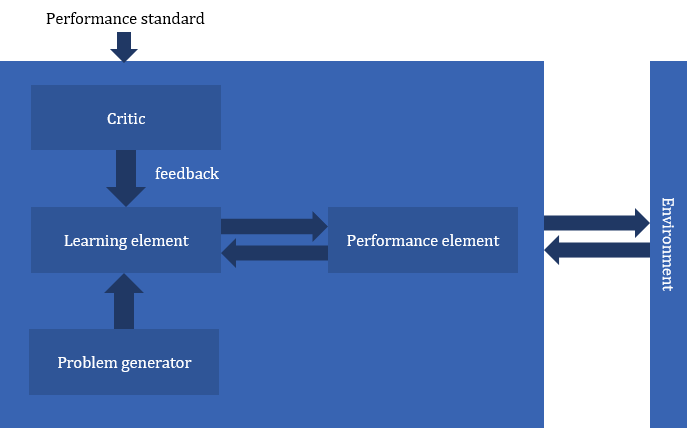
\includegraphics{aima_learning_agent}
    \centering
    \caption{An overview schematic of the learning agent system.}
    \label{fig:aima-learning-agent}
\end{figure}

\subsubsection{Learning and Performance}
The performance elements provides the basic function of the agent: it perceives, decides and acts.
The learning element's job is to improve this performance based on feedback, coming from an outside observer (the critic).
The learning element's design varies depending on the problem and how the agent is meant to interact with it.

\subsubsection{Critics}
An agent cannot tell whether its behaviour is effective just by observing changes in the environment.
It needs a \textbf{critic} that provides feedback to the learning element about its performance in the world.
The critic can esentially be viewed as a stand-alone, external entity.
It is based on a fixed performance standard which does not depend on the agent's internal state.
In fact, it is imperative for the critic to be kept separate of agent state.
This prevents the agent of ``deluding'' itself that it is doing a good job.

\subsubsection{Problem Generators}
Agents can get stuck making decisions that yield good but suboptimal results (local optima, a well-known problem in AI).
This happens because the agent bases its calculations on limited knowledge.
It needs a component to take care of adding new information into its system.
The problem generator solves this problem of \textbf{exploration}:
choosing options that yield suboptimal results in the short term, in order to discover better strategies on the long term.

\clearpage  % put here to push the RL chapter onto the next page instead of having 2 lines dangling there

\section{Reinforcement Learning} \label{reinforcement-learning}
\textbf{Reinforcement learning (RL)} is an area of machine learning that epitomizes the agent-based approach.
RL is unique within its field as it is directly focused on goal-directed learning from agent-environment interaction \cite{rlai}.
At the core of RL lays the reward function (or signal), which perfectly describes goals established by the problem.

In the following chapter, we start by summarizing finite MDPs -- the mathematical underpinning for reinforcement learning, while also familiarizing with the the notation used throughout this paper.

In section \ref{rl:dp} we cover the first solution technique: using dynamic programming in a known, finite MDP to find its optimal solution.
In section \ref{rl:mc}, we generalize this method to solve unknown MDPs -- the complete formulation of a RL problem -- using Monte-Carlo learning.
In section \ref{rl:td}, we visit temporal-difference learning and finally develop our solution using Q-learning in section \ref{rl:q-learning}.

\subsection{Components and Notation}
Introduction into reinforcement learning supposes familiarity with the paradigm's simple-but-effective mathematical framework.
We present the theory behind Markov decision processes (MDPs) and then we shift our attention to explaing the components of a reinforcement learning agent.

\subsubsection{Finite Markov Decision Processes}
Finite Markov decision processes are a formalization of a reinforcement learning problem -- any problem which can be represented as a finite MDP can be solved using a RL technique.

The feedback loop is central to understanding the reinforcement learning dynamic.
This is just a reiteration of the contents in our previous chapter:
an \textbf{agent} acts upon an \textbf{environment}, which reacts according to its set of governing rules.
Each iteration takes place at a discrete time step \(t = 0,1,2,\dots \) (although there are continuous variants of a Markov process, we are not concerned with them).

\begin{figure}[ht]
    \centering
    \caption{Feedback Loop. (Partial reproduction from \cite{rlai})}
    \vspace*{0.2cm}
    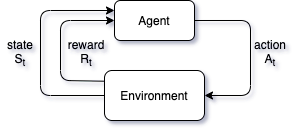
\includegraphics[width=0.5\textwidth]{agent-env-fig}
\end{figure}

\begin{enumerate}
    \item The agent is in state \(s\) and picks action \(a\).
    \item It receives a reward \(r\) for its action. This (immediate) reward signal is problem-defined and quantifies the agent’s goal.
    \item The environment reacts, sending the agent into the next state \(s'\).
\end{enumerate}

A \textbf{Markov decision process (MDP)} is defined as a tuple \(\langle S, A, P, R, \gamma \rangle\), in which:
\begin{enumerate}
    \item \(S\) is the finite set of all states.
    \item \(A\) is the finite set of all possible actions.
    \item \(P\) is the state transition probability function, where \(P_a(s, s')\) denotes the probability of starting in state \(s\) and ending up in state \(s'\) by taking action \(a\).
    \item \(R\) is the reward function, where \(R_a(s, s')\) is a value in \(\mathbb{R}\) and represents the reward received for starting in state \(s\) and ending up in state \(s'\) by taking action \(a\).
    \item \(\gamma\) is the discount factor (used when computing the \textbf{return}), \(\gamma \in [0, 1]\).
\end{enumerate}

The \textbf{state} refers to the internal state of the agent \footnote{Sometimes we may also refer to the state of the environment, but context will clarify. Environment state and agent state only completely match in full observability environments.}.
A state \(S_t\) contains relevant information from the environment at a given time step \(t\).
A key point in Markov processes is that a correctly formulated state captures all the relevant information and removes the need of explicitly memorizing state history.
This is known as the \textbf{Markov property} \cite{silver-lectures}.

A \textbf{policy \(\pi\)} completely characterizes an agent’s behaviour.
``It is a mapping from perceived states of the environment to actions to be taken in those states'' \cite{rlai}.
Policies can be deterministic (i.e. ``if this then that'' rules) or stochastic.
A \textbf{stochastic policy}, denoted \(\pi(a \given s)\), is a probability distribution over actions, given a state.

The \textbf{reward} models the problem-defined goals as a scalar that can be associated with each state transition.
``The reward signal is the primary basis of altering the policy.'' \cite{rlai}.
The assertion that we can completely and correctly model all goals using reward functions is central to the field of RL.
This is called the \textbf{Reward Hypothesis} and is formulated below:
\begin{quotation}
    That all of what we mean by goals and purposes can be well thought of as maximization of the expected value of the cumulative sum of a received scalar signal (called reward). \textit{(from \cite{rlai}, Chapter 3.2)}
\end{quotation}

The \textbf{return} \(G_t\) is the \textbf{cumulative reward} obtained by the agent starting from time step \(t\).
This is what a reinforcement learning system is supposed to maximize.
There are multiple mathematical models used to represent the return.
In equation \ref{eqn:return}, we use an infinite-horizon sum with discounting.

\begin{equation} \label{eqn:return}
    G_t = R_{t+1} + \gamma R_{t+2} + \dots = \sum_{k = 0}^{\infty}{\gamma^{k} R_{t + k + 1}}    
\end{equation}

Discounting is, intuitively, a way to control how much the agent cares about future rewards.
More on this topic can be found in either theoretical reference \cite{rlai, silver-lectures}.

% todo: explain why discounting is used and why it is convenient

\subsubsection{Value Functions} \label{rl:value-func}
The \textbf{state-value function} for policy \(\pi\) is denoted by \(V^{\pi}(s)\) and measures how good each state is, with regard to the long-term potential of that state.
Whereas rewards characterize the immediate value of a state, the value function measures its long-term desirability \cite{rlai}, under the given policy.

\begin{equation} \label{eqn:value}
    V^{\pi}(s) = \mathbb{E}_{\pi}\{ G_t \given S_t = s \}
\end{equation}

In Equation \ref{eqn:value}, \(\mathbb{E}\) represents the expected value of a random variable. Here we are interested in the expected value of the return, or simply -- the \emph{expected return}.
By \(\mathbb{E}_{\pi}\) we denote the expected value conditional on following policy \(\pi\).
We will maintain this notation in the expressions below.

The \textbf{action-value function} \(Q^{\pi}(s, a)\), also known as the Q-value function, measures the desirability of a state-action pair.
More explicitly, it gives the expected return of starting in state $s$ and taking action $a$, then continuing to follow policy $\pi$.

\begin{equation}
    Q^{\pi}(s, a) = \mathbb{E}_{\pi}\{ G_t \given S_t = s, A_t = a \}
\end{equation}

Action-value functions are especially important in \textbf{model-free methods} (see \emph{Models} in Section \ref{rl:model}), which are predominantly the focus of this paper.
In model-based algorithms, the value function $v$ can uniquely determine a policy: we can simply pick the best reward-state pair.
This naturally requires knowing the full dynamics of the MDP (knowing all successor states of $s$).

However, for many tasks, especially those relevant in the real-world, it is impractical (if not impossible) to know or to model the environment.
Keeping track of both \emph{states and actions} allows model-free learning algorithms to construct policies without knowledge of environment dynamics.

\subsubsection{Optimal Value Functions}

There are optimal variants of the same value functions.
In order to understand the concept of \textbf{optimality}, we need to define an \textbf{ordering} between policies.
Considering $\pi$ and $\pi'$, we say that $\pi' \geq \pi$ if $V^{\pi'}(s) \geq V^{\pi}(s)$ for every $s \in S$.
Using this definition, we can say that there exists a $\pi^{*}$ which is the \textbf{optimal policy}, being greater than or equal to all other possible policies.

The \textbf{optimal value function $V^*(s)$} represents the maximum value obtained in state $s$, over all policies, as briefly summed up the relation below.

\begin{equation} \label{eqn:opt-value-fun}
    V^*(s) = \max_{\pi}{V^{\pi}(s)}
\end{equation}

Similarly, \textbf{optimal action-value function $Q^*(s, a)$} is the maximum value of being in state $s$ and taking action $a$, considered over all policies.

\begin{equation} \label{eqn:opt-Q-fun}
    Q^*(s) = \max_{\pi}{Q^{\pi}(s, a)}
\end{equation}

Value function approximation is the foundation of multiple solution methods in RL.
A simple example can be seen in Monte Carlo methods, where the value of a state \(s\) is approximated by averaging over multiple trajectories starting from \(s\).

\subsubsection{Models} \label{rl:model}
A \textbf{model} (of the environment) allows the agent to plan and make predictions of its environment.
Some algorithms focus explicitly on learning a model and use it for \textbf{planning}.
This approach is called \textbf{model-based}.
In a model-based method, an agent can query the model to simulate what would happen with the environment before actually choosing an action.
Approaches without a model are called \textbf{model-free}. Model-free agents are ``explicitly trial-and-error learners'' \cite{rlai}.

\begin{figure}[ht]
    \caption{A way of classifying RL methods based on whether they have a value function, policy or model. (Reproduced from David Silver's lectures. \cite{silver-lectures})}
    \vspace*{0.2cm}
    \centering
    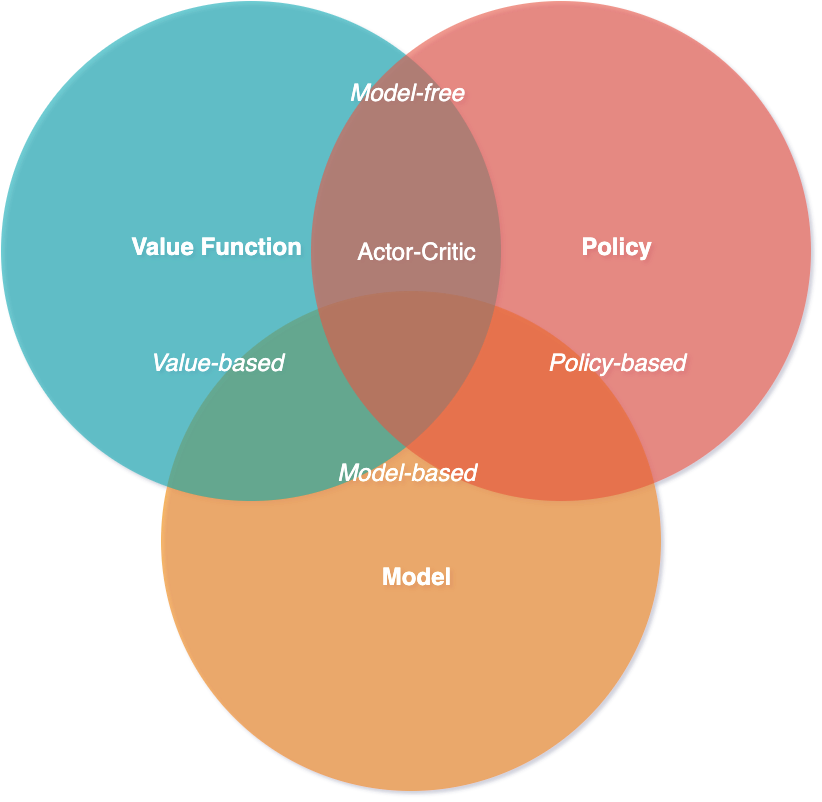
\includegraphics[width=0.5\textwidth]{silver-venn}
\end{figure}

\subsection{Bellman Equations} \label{rl:bellman}
The \textbf{Bellman equations} are a set of relations conceived by Richard Bellman in the 1950s, in the context of solving optimal control using dynamic programming.
In the reinforcement learning context, they interrelate the state-value and action-value functions and provide the basis of solving an MDP whether known or unknown.

Equation \ref{eqn:bellman-expectation} states the \textbf{Bellman expectation equation}.
The key idea behind this class of Bellman equations is that they express the value of a state as expected sum of immediate reward of being in that state,  plus discounted value of successor state.
This transformation becomes clear if we use our return-based exprimation of value function $V^{\pi}(s)$ in Equation \ref{eqn:value} and reorganize its terms:

\begin{equation} \label{eqn:bellman-expectation}
\begin{aligned}
    V^{\pi}(s)
        &= \mathbb{E}_{\pi}\{ G_t \given S_t = s \} \\
        &= \mathbb{E}_{\pi}\{ R_{t+1} + \gamma R_{t+2} + \dots \given S_t = s \} \\
        &= \mathbb{E}_{\pi}\{ R_{t+1} + \gamma V^{\pi}(S_{t+1}) \given S_{t} = s \} \\
\end{aligned}
\end{equation}

In Figure \ref{fig:expectation-backup}, we model the equation using a backup tree\footnote{Called a backup or update tree, it visualizes the way that state values are updated. This visualization convention is proposed in and used throughout \cite{rlai}.}, where each open circle represents a state, while closed cicles represent state-action pairs.

In state $s$, the agent has a set of available actions according to its policy $\pi$.
After the agent chooses action $a$, the environment responds with reward $r$ and throws the agent into the next state  $s'$ -- one of multiple possible states according to environment dynamics.

Equation \ref{fig:expectation-backup} computes the value of state $s$ by \emph{averaging} over all possible trajectories, \emph{weighing} each by its probability of occuring.

\begin{figure}[ht]
    \centering
    \caption{Bellman expectation backup.} \label{fig:expectation-backup}
    \vspace*{0.2cm}
    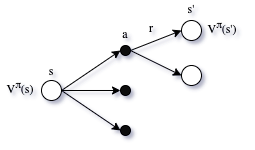
\includegraphics[width=0.4\textwidth]{bellman-expectation-backup}
\end{figure}

In cases in which the MDP is \emph{known}, we can leverage the fact that we know the transition probabilities $P$ to \emph{directly compute} the expectation in \ref{eqn:bellman-expectation}.
\begin{equation}
    \begin{aligned}
        V^{\pi}(s)
            &= \mathbb{E}_{\pi}\{ R_{t+1} + \gamma V^{\pi}(S_{t+1}) \given S_{t} = s \} \\
            &= \sum_{a \in A}{
                \pi(a \given s) ( R(s, a) + \gamma \sum_{s' \in S}{
                    P_a(s, s') V^{\pi}(s')
                })
            }
    \end{aligned}
\end{equation}

There exists another relation with important applications in RL -- the \textbf{Bellman optimality equation}.
One way of expressing the optimality equation, provided in \ref{eqn:bellman-optimality}, simply states the fact that the optimal value of a state must be the value of the best possible action from that state \cite{rlai}.
This is an example of interdependence of the two value functions, although it is important to mention that we can express $q_{*}$ in terms of itself as well.

\begin{equation} \label{eqn:bellman-optimality}
    \begin{aligned}
        v_*(s) = \max_{a \in A} q_{*}(s, a)
    \end{aligned}
\end{equation}

The optimality equation is non-linear, but we cover approximating solutions using iterative methods in our dynamic programming section at \ref{rl:dp}, specifically to solve planning problems (which require finding the optimal policy).

\subsection{Dynamic Programming} \label{rl:dp}
\textbf{Dynamic programming (DP)} methods are an important theoretical starting point for reinforcement learning methods. DP problems require full knowledge of an MDP and use general methods to compute optimal solutions.

While being theoretically useful, there are key bottlenecks which prevent DP from achieving practicality:

\begin{enumerate}
    \item DP represents a \textbf{subset} of a reinforcement learning problem, as it requires full knowledge of an MDP and, thus, is not suitable in unknown environments.
    \item DP is \textbf{computationally expensive} as it searches for optimal solutions over the entire state space (suffers from the ``curse of dimensionality'' \cite{rlai}).
    \item DP cannot be applied with \textbf{continuous} spaces, unless problems satisfy additional criteria \cite{rlai}.
\end{enumerate}

There are two key problems that can be solved using DP in a fully known MDP using the Bellman equations.

\textbf{Policy evaluation}, also reffered to as \emph{prediction}, starts with a given policy $\pi$ and is concerned with finding its value function $v_{\pi}$.
In theory, the value of each state can be computed by solving a system of Bellman equations, one for each state.
However, the computation required is impractical for most problems.
A more suitable method is \emph{iterative policy evaluation}, which uses equation \ref{eqn:bellman-expectation} iteratively, starting from an arbitraty value function $v_0$ and eventually converging to $v_{\pi}$.

\textbf{Control} (or \textbf{planning}) is, in constrast, concerned with finding the optimal policy $\pi^{*}$ starting from an arbitraty point in the space.

Planning can be done using \emph{policy iteration}.
At every iteration $k$, this method evaluates the given policy $\pi$ to find its value function $v_{\pi}$ (solving the above problem).
Then, it constructs a new policy $\pi'$ which acts \emph{greedily} with regard to $v_{\pi}$.
This is proven to eventually converge to $\pi^*$ as $k \to \infty$ \cite{rlai}.

\begin{figure}[h]
    \caption{An illustration of policy iteration. (From David Silver's lectures. \cite{silver-lectures})}
    \centering
    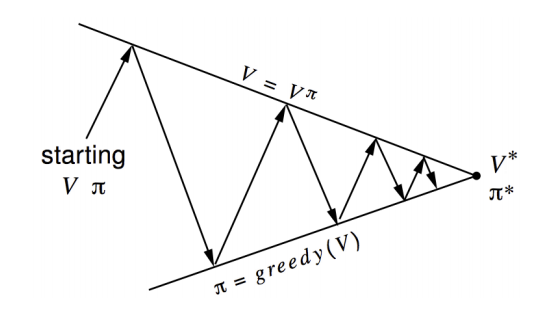
\includegraphics[width=0.4\textwidth]{silver-policy-iteration}
\end{figure}

Using policy iteration can be extremely expensive, as the method adds an additional layer of computation on top of already costly policy evalutation.
The idea of \textbf{value iteration} comes from collapsing the evaluation step with the policy construction step, by applying ``one sweep'' policy iteration -- only updating each value once at every step.

\subsubsection{Generalized Policy Iteration (GPI)}
As we have seen so far, policy iteration consists of two simultaneous, interacting processes \cite{rlai}: policy evaluation and policy improvement.
Different algorithms interrelate the two phases in different ways, e.g. value iteration performs one sweep of policy evaluation while vanilla policy iteration goes through to the end.

\textbf{Generalized policy iteration} is a broad framework specifying only that policy evaluation and policy iteration are used alongside each other, abstracting the exact details of their interaction.
Most reinforcement learning algorithms can be described by GPI at the high-level.

\clearpage

\subsection{Monte Carlo Learning} \label{rl:mc}
In reinforcement learning, Monte Carlo is a family of methods that learn from complete episodes of experience by sampling average returns.
The term “Monte Carlo” is broadly used in mathematics to mean any evaluation method that involves a significant random component \cite{rlai}.

\begin{figure}[ht]
    \caption{Backup tree for Monte Carlo, highlighting a sample episode up to its terminal state. (From David Silver's lectures. \cite{silver-lectures})}
    \centering
    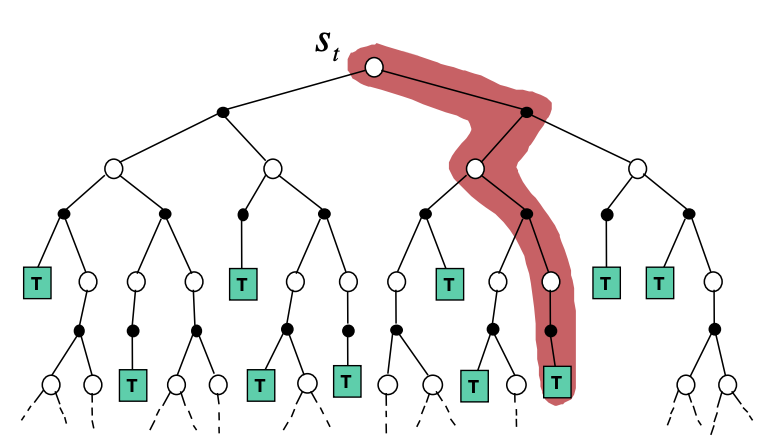
\includegraphics[width=0.5\textwidth]{montecarlo-backup.png}
\end{figure}

Monte Carlo approximates the expected return of any given state by averaging over the set of \emph{episodic returns} for that state.
For this, we interact with the environment over multiple episodes, with the condition that every episode \emph{eventually terminates}, independently of the actions taken by the agent.
Eventual termination is necessary for all returns to be well-defined.

Monte Carlo introduces one of the missing pieces required to solve model-free problems -- \textbf{sampling}.
Below, we describe a simplified, general version of the algorithm to better illustrate the approach.
Each state holds a variable $count(s)$, the number of first-visits (or every-visits) over the set of all sampled episodes, as well as a $sum(s)$ -- the sum of returns over this set of samples.

The value of a state $v(s)$ can then be approximated as the mean over all obtained returns, $sum(s) / count(s)$.
Given the law of large numbers, $v(s)$ will eventually converge to the correct values as the number of episodes approaches infinity.

\subsubsection{Monte Carlo Control}
Monte Carlo addresses the \textbf{complete} reinforcement learning problem, as it only requires episodes of experience to learn the optimal solution, in contrast to DP, which requires a fully known model of the environment.

Thus far, we presented Monte Carlo as a viable strategy for policy evaluation in unknown environments (\emph{model-free prediction}).
In order to apply this for \textbf{control} problems, we use the General Policy Iteration (GPI) framework, drawing upon what we discussed in Section \ref{rl:dp}, \emph{Dynamic Programming}.

\begin{figure}[h]
    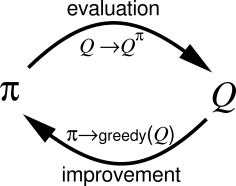
\includegraphics[width=5cm]{montecarlo-gpi.png}
    \centering
    \caption{Monte Carlo control using the GPI framework. (From \cite{rlai})}
\end{figure}

Applying this pattern, we can use Monte Carlo estimation as the \emph{prediction} step to approximate the optimal policy, thus obtraining Monte Carlo \emph{control}.
Using action-value functions (which are required in unknown environments, as mentioned in our section on value functions), the policy improvement step is simply done by choosing the action yielding the maximum value.

\begin{equation}
    \pi(s) = \argmax_{a \in A}{Q(s, a)}
\end{equation}

\subsubsection{Exploration and Soft Policies}

Besides the termination requirement, Monte Carlo control will not converge to any useful solution unless efficient \textbf{exploration} of the state space is guaranteed.
For this purpose, we introduce the notion of a \textbf{soft policy}.

Soft policies guarantee that we do not permanently exclude any state from our search, or -- in other words -- that $\pi (s, a) > 0$ for all $s \in S$ and $a \in A$.
\textbf{$\varepsilon$-greedy policies} are commonly used for this purpose.
Under an $\varepsilon$-greedy policy, $\varepsilon \in (0, 1]$ is the probability of choosing a random action in any state instead of acting greedily.

\subsection{Temporal-Difference Learning} \label{rl:td}
\textbf{Temporal-difference (TD) learning} is a class of model-free algorithms that are able to learn from incomplete episodes.
Compared to Monte Carlo, TD methods (being model-free) similarly learn by sampling from the environment, but differ through the fact that they do not require complete episodes of experience.

There exist advanced generalizations of the simple TD algorithm, such as TD($\lambda$), but they are outside the scope of this paper.
Here we will only cover the case of one-step TD learning, known in \cite{rlai} as TD(0).

\subsubsection{Bootstrapping}
Similar to the dynamic programming approach, TD updates the value function based on previous estimations of itself.
This is called \textbf{bootstrapping} and can be intuitively described as the idea of \emph{learning a guess from a guess} \cite{rlai}.

\begin{figure}[h]
    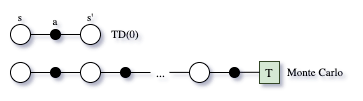
\includegraphics[width=0.7\textwidth]{td-mc-backups.png}
    \centering
    \caption[Caption]{Backup tree for one update step of TD(0) next to one update step of every-visit Monte Carlo.} \label{fig:td-mc-update-steps}
\end{figure}

In Figure \ref{fig:td-mc-update-steps}, an \emph{update step} is not a time-step but instead refers to an iteration of each algortihm.
In the case of TD(0), the terms do correspond, as the update can be performed after each time-step.
For Monte Carlo, the update is run only after the end of each episode.

The concept can be generalized to $n$-step bootstrapping (updating after $n$ steps instead of one).

Temporal-difference solves the same \textbf{prediction} problem as Monte Carlo.
In this section we contrast the two approaches and establish the definition of the TD target and the TD error.

We consider a Monte Carlo approach where we update $V^{\pi}(s)$ towards the return $G_t$ softly at the end of each episode, considering a learning rate of $\alpha \in (0, 1)$.
This Monte Carlo backup operation is given by Equation \ref{eqn:td-mc} \cite{rlai}.

\begin{equation} \label{eqn:td-mc}
    V(S_t) \leftarrow  V(S_t) + \alpha[G_t - V(S_t)]
\end{equation}

Observe how in Monte Carlo, we update at the end of an episode and so we know the return $G_t$ exactly -- this is our \emph{ground truth}.
In TD, the rewards themselves provide a stable ground, but the values are adjusted towards our \emph{best guess} (the value from our previous iteration).

\begin{equation} \label{eqn:td-td}
    V(S_t) \leftarrow  V(S_t) + \alpha[
        \overbrace{\underbrace{R_{t+1} + \gamma V(S_{t+1})}_\text{TD target} - V(S_t)}^\text{TD error}
    ]
\end{equation}

Equation \ref{eqn:td-td} describes the update step in temporal-difference learning.
We define the \textbf{TD target} according to the Bellman expectation equation -- $\delta = R_{t+1} + \gamma V(S_{t+1})$.
After each step of experience, the current value is adjusted softly towards the \textbf{TD error} which is simply $\delta - V(S_t)$.

\textbf{TD control}, like Monte Carlo control, uses GPI with TD as the prediction step.
Control algorithms are split into two distinct classes: on-policy and off-policy algorithms.
We explain the difference between the two, then focus on the off-policy TD case (Q-learning, in Section \ref{rl:q-learning}).

\subsection{On-Policy and Off-Policy Control}
In control algorithms, we can distinguish two different types of policies.
\begin{enumerate}
    \item The \textbf{target policy} is the policy which the algorithm estimates or optimizes -- this type, whether explicitly or implicitly, is present in all RL algorithms.
    \item The \textbf{behaviour policy} (sometimes denoted by $\mu$) is the policy effectively followed by the agent, i.e. it is directly used to choose actions in the environment.
\end{enumerate}

The class of algorithms which uses a behaviour policy $\mu$ in order to learn about a \emph{separate} target policy $\pi$ is called \textbf{off-policy}.
Off-policy agents try to learn optimal behaviour by observation of exploratory behaviour.

The alternative strategy is \textbf{on-policy} learning, in which the learned policy coincides with the behaviour policy.
On-policy learning agents learn ``on the job'' \cite{silver-lectures}, i.e. evaluate a policy by acting according to that policy.

Off-policy approaches are suitable for learning from knowledge generated by human experts or by other agents, including non-intelligent agents.
They are more desirable \emph{in general}, as on-policy agents tend to learn suboptimal behaviours in order to counteract the effects of exploration (as can be seen from the \emph{Example 6.6. Cliff Walking}, given in \cite{rlai}).

Despite being generally more useful, off-policy learning introduces \textbf{additional complexity} because it needs additional guarantees.
Off-policy learning assumes that behaviour policy $\mu$ has \textbf{coverage} of the target policy $\pi$ \cite{rlai}.
Coverage implies that $\mu$ visits all state-action pairs that would be visited by $\pi$.

% This would be a good place to plug-in and explain Cliff Walking in detail.
% in that case, this should break off and become its own section

TD learning contains strategies aligning with both categories: Sarsa is an on-policy TD control algorithm, while Q-learning is its off-policy counterpart.

\subsection{Q-learning} \label{rl:q-learning}
\textbf{Q-learning} \cite{Watkins1992} an off-policy TD learning algorithm considered one of the early breakthroughs of RL.
Its rather non-descriptive name comes from the action-value function $Q$ (which itself stands for ``quality'').

Q-learning learns an optimal policy by following an $\varepsilon$-greedy exploratory policy.
The principle underneath, however, can be adapted to learn from any other policy as long as the coverage property is respected.
Q-learning achieves coverage, since a greedy policy is ``included'' into its $\varepsilon$-greedy counterpart.

At each step, the algorithm bootsraps using the maximum action-value over the next state in order to better estimate current state value.
The update rule is represented in Figure \ref{fig:q-learning-backup}.
The arc over the set of successor states represents the maximization (greedy) operation.

\begin{figure}[h]
    \centering
    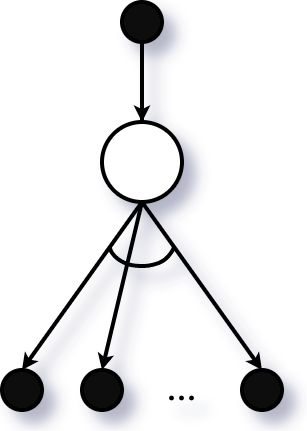
\includegraphics[width=3cm]{q-learning-backup.png}
    \caption{Q-learning backup diagram.}
    \label{fig:q-learning-backup}
\end{figure}

The same rule is mathematically represented in Equation \ref{eqn:q-learning-update-rule}.
It follows the TD learning pattern presented in Equation \ref{eqn:td-td}. Here, our \textbf{TD target} uses the maximum successor Q-value -- $\delta = R_{t+1} + \gamma \max_{a \in A}{Q(S_{t+1}, a)}$.


\begin{equation} \label{eqn:q-learning-update-rule}
    Q(S_t, A_t) \leftarrow Q(S_t, A_t) + \alpha [
        R_{t+1} + \gamma \max_{a \in A}{Q(S_{t+1}, a)} - Q(S_t, A_t)
    ]
\end{equation}
 
\pagebreak

\section{Deep Reinforcement Learning} \label{deep-rl}
Researchers found that advances in the field of deep learning -- a broad family of methods based on artificial neural networks -- can be used to enhance the classical RL algorithms.
This led to the expansion of the field, marking the birth of \textbf{deep reinforcement learning (deep RL)}.

Classic RL assumes that the state space is finite and can be modeled in a tabular manner.
However, we seldom encounter real-world, interesting problems where this assumption holds.
Deep RL is an open field striving to solve \emph{more complex} problems than classical methods allow.
This is done through the ability of functional approximators to model high-dimensional spaces.

The field has recently surged, after a series of new algorithms and succesful applications were published.
In this chapter, we try to give an overview of the main methods of learning but mainly focus on developing \emph{Mnih et al.'s \textbf{DQN} (2013)} \cite{atari-dqn}.

In Section \ref{section:convnets}, we present \textbf{convolutional neural networks}, a class of artificial neural networks which became the foundation of multiple algorithms in deep RL.

Section \ref{section:dqn} covers using neural networks (called deep Q-networks in the paper \cite{atari-dqn}) as approximators in Q-learning in order to build autonomous agents for complex model-free environments.

The rest of the chapter (Sections \ref{section:policy-opt} and \ref{section:actor-critic}) deals with alternative strategies for doing (deep) model-free control, namely \textbf{policy optimization} and \textbf{actor-critic} methods respectively.

\clearpage

\subsection{Convolutional Neural Networks (ConvNets)} \label{section:convnets}
\textbf{Convolutional neural networks} (often shortened as ConvNets or CNNs) are a specific type of artificial neural network for processing data that has a known grid-like topology \cite{Goodfellow-et-al-2016}.

ConvNets exploit the \textbf{spatial nature} of the data.
This property makes them especially useful over a vast spectrum of problems, such as image classification, audio signal processing, analyzing financial time-series etc.
Among those, image classification tasks are the primary reason for the architecture's popularity.

The \textbf{origin} of convolutional networks can be traced back to Kunihiko Fukushima's \emph{neocognitron} (1979).
Kunihiko’s design \cite{neocognitron-paper} was itself inspired by earlier breakthroughs in neuroscience -- namely studies of the visual cortex of mammals (Hubel \& Wiesel, 1959).
LeCun et al. (1989) further improved this model by introducting backpropagation training, which set the standard for today’s architectures.

\subsubsection{Overview}
A convolutional network contains at least one convolutional layer in its structure.
A typical convolutional layer (represented in Figure \ref{fig:conv-layer}) is composed of three stages \cite{Goodfellow-et-al-2016}:
\begin{enumerate}
    \item The \textbf{convolution stage} convolves the input data with a filter (kernel), which results in a set of linear activations.
    The kernel is the learned element, i.e. we learn the weights of the kernel as we would learn the weights of a linear layer.
    \item The \textbf{detector stage} pipes each linear activation from the convolution layer thorugh a non-linear activation function (e.g. ReLU \footnotemark)
    \item The \textbf{pooling stage} is an optional stage which reduces the output size by computing summary statistics over the data.
\end{enumerate}
\footnotetext{standing for \emph{rectified linear unit}, it is commonly used as an activation function in neural networks. In its classic form, it can be expressed as $f(x) = max(0, x)$.}

\begin{figure}[h]
    \centering
    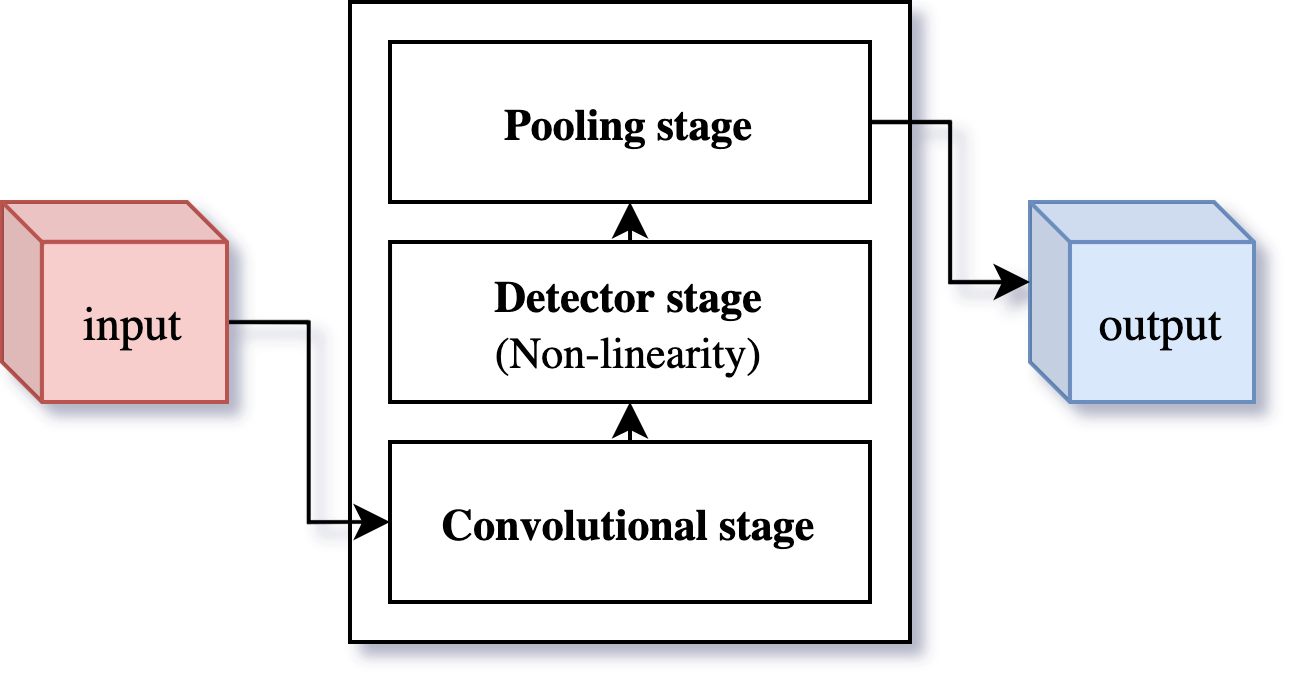
\includegraphics[width=0.7\textwidth]{conv-layer-structure.png}
    \caption{A schematic of a convolutional layer.}
    \label{fig:conv-layer}
\end{figure}

In this section, we consider the \textbf{input} and \textbf{output data} to be 3D tensors, consisting of a spatial dimension (width and height) and a depth dimension.
Visualizing this process with images in mind is particularly helpful to understanding.
The spatial dimensions map exactly to the width and height of an image, and each color channel can be considered a separate depth level.


\subsubsection{The Convolutional Stage}
This stage performs the convolution operation which is the most computationally demanding procedure of the layer.
The output from this stage is a \textbf{feature map} of the input, which is then passed as linear activation to the detector stage, likewise to fully-connected feedforward networks.

This \textbf{operation} consists of sliding a \emph{kernel} over the input.
At every step, we compute the dot product between the kernel and the volume of input it currently overlaps.
The \textbf{kernel} (or filter) is a tensor of adjustable weights, which is small relative to the image's spatial dimentions but must cover the entire depth of the image.
The effects of the convolutional stage are determined by a number of hyperparameters: depth, stride and padding.

A convolutional stage can learn multiple independent kernels.
The number of kernels is given by the \textbf{depth} hyperparameter.
It is conveniently called such because it corresponds to the depth of the output of this stage.
A \textbf{depth column} (or fibre) \cite{stanford-convnets} is a set of neurons ``looking'' to the same region in the input (where each neuron corresponds to a different kernel) .

The \textbf{stride} specifies the distance which we slide the kernel with over the input at each step.
Some models provide separate stride parameters for each axis (horizontal and vertical) \cite{Goodfellow-et-al-2016}.

\textbf{Zero-padding} (or simply padding) enables padding our input data with zeros along the borders. It is useful for controlling output size, especially in cases where we want to preserve the input size over multiple layers.

\begin{figure}[h]
    \centering
    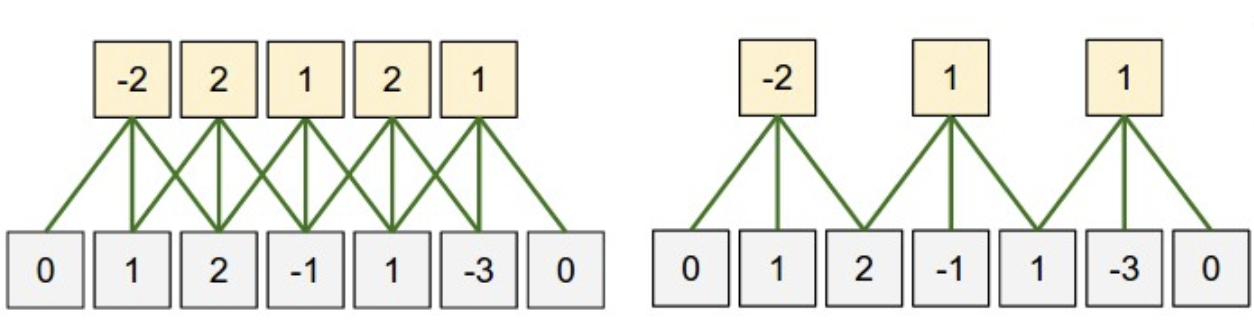
\includegraphics[width=0.6\textwidth]{conv-stride-padding.png}
    \caption{(Left) Using a stride of 1 and a zero-padding of 1 to preserve the original spatial dimensions of the input. (Right) Using a padding of 1 and a stride of 2, which results in fewer output values. (Illustration from \cite{stanford-convnets})}
    \label{fig:conv-stride-padding}
\end{figure}
 
The properties of convolution confer ConvNets a myriad of advantages over fully-connected feedforward neural networks.
This gain in efficiency comes from the assumption that the data has an underlying spatial structure, which can be exploited better by ConvNets than by alternatives.

Typical fully-connected layers relate all their outputs to all their inputs by separate, \emph{independently adjustable} weights.
This requires storing weight matrices as large as the input data itself, rising the computational cost as input size grows.
In contrast, kernels are significantly smaller than the input volume is (in the spatial dimensions).
Kernels are also reused across the entire layer (\textbf{parameter sharing}), resulting in smaller memory requirements.

ConvNets feature \textbf{sparse interactions}, in contrast to the dense interactions of fully-connected layers in which every output is related by a weight to each of the input values.
This boost learning efficiency by reducing the number of necessary computations.

Learning smaller, shared kernels can be a means of controlling \emph{overfitting} \cite{Goodfellow-et-al-2016}. Moreover, ConvNets can operate on input data of \textbf{varying sizes} without making adjustments to model architecture.


\subsubsection{Pooling}
The \textbf{pooling stage} is an optional stage in the ConvNet architecture which performs a \emph{downsampling} of its inputs.
The role of this stage is to gradually reduce computation (and memory requirements) in the network by reducing the spatial dimension of the data \cite{stanford-convnets}.
It usually processes output from the convolutional stage to which it applies a pooling function.

A \textbf{pooling function} computes a summary statistic (e.g. maximum, average, $l^2$-norm etc.) over a neighbourhood of input values \cite{Goodfellow-et-al-2016}.
The pooling stage has a similar operation to the convolutional stage:
a moving window is slided over and across the input data and at each step, the summary is computed.

Each depth slice of the data is processed independently.
An example for a simple but commonly use operation (max pooling) is shown in Figure \ref{fig:maxpooling}.

\begin{figure}[h]
    \centering
    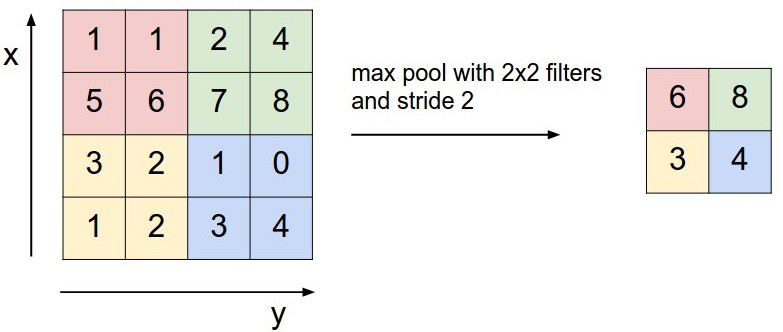
\includegraphics[width=0.8\textwidth]{conv-maxpooling.jpg}
    \caption{Simple example illustrating max pooling (on a single depth level). Illustration from \cite{stanford-convnets}.}
    \label{fig:maxpooling}
\end{figure}

\subsection{Deep Q-Networks (DQN)} \label{section:dqn}

\subsection{Policy Optimization Methods} \label{section:policy-opt}

\subsection{Actor-Critic Methods} \label{section:actor-critic}
